\section{Numerical simulations}


\begin{frame}{Numerical simulations}
	\framesubtitle{MSS Toolbox}
	The Marine Systems Simulator (MSS) is a Matlab and Simulink library for marine control systems design. The m-files are compatible with the free software GNU Octave. MSS includes models for ships, underwater vehicles, uncrewed surface vehicles, and floating structures. The library also contains guidance, navigation, and control (GNC) blocks for time-domain simulation. 
	
	\vspace{6cm}
	
	\begin{tikzpicture}[remember picture,overlay]
		% \node[fill=blue!30, text=white, font=\large, rounded corners] 
		\node at (current page.north west) [xshift=4cm, yshift=-6cm] {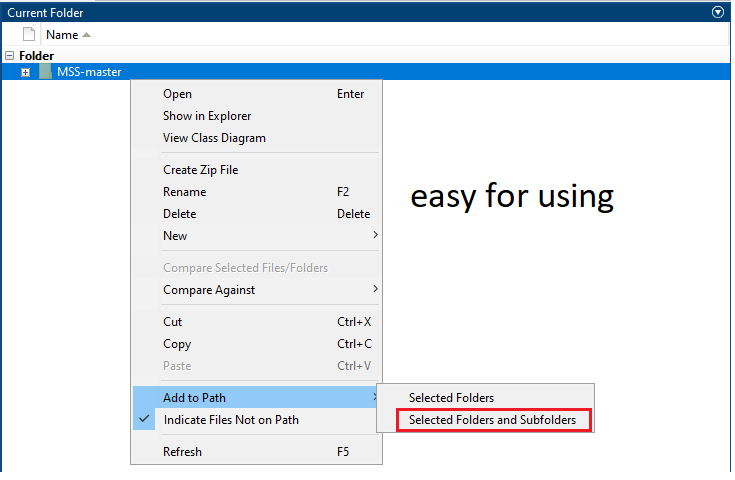
\includegraphics[width=0.5\linewidth]{img/addpath.png}};
	\end{tikzpicture}
	
	
	\begin{tikzpicture}[remember picture,overlay]
		% \node[fill=blue!30, text=white, font=\large, rounded corners] 
		\node at (current page.north west) [xshift=9.5cm, yshift=-6.3cm] {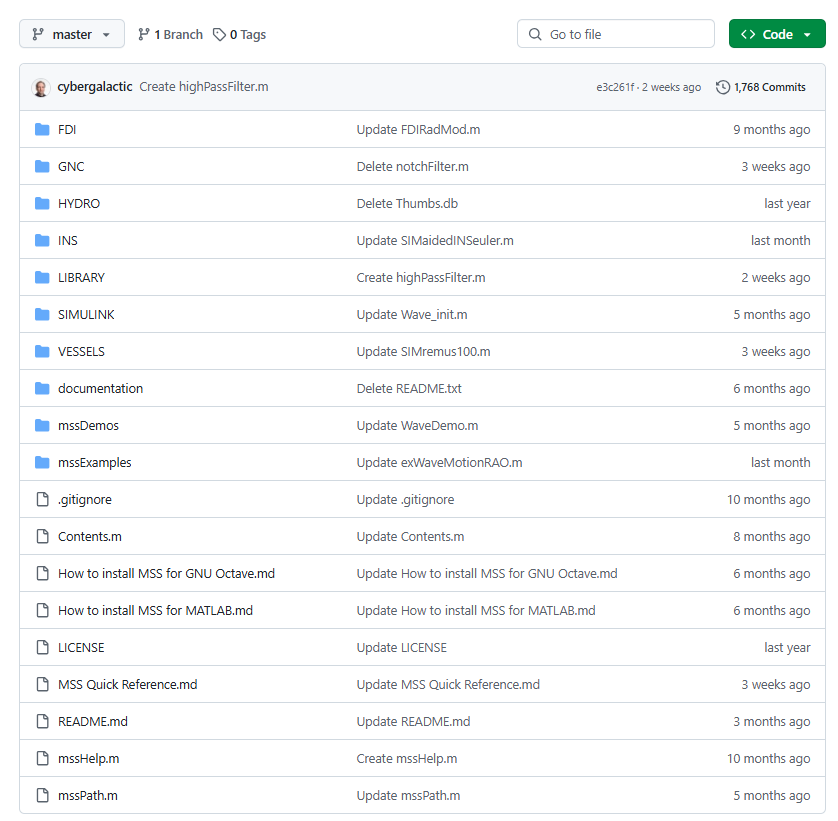
\includegraphics[width=0.5\linewidth]{img/mss_github.png}};
	\end{tikzpicture}
\end{frame}



% =========================================
% =========================================


\begin{frame}{Numerical simulations}
	\framesubtitle{MSS Toolbox}
	The Marine Systems Simulator (MSS) is a Matlab and Simulink library for marine control systems design. The m-files are compatible with the free software GNU Octave. MSS includes models for ships, underwater vehicles, uncrewed surface vehicles, and floating structures. The library also contains guidance, navigation, and control (GNC) blocks for time-domain simulation. 
	
	\vspace{6cm}
	
	\begin{tikzpicture}[remember picture,overlay]
		% \node[fill=blue!30, text=white, font=\large, rounded corners] 
		\node at (current page.north west) [xshift=3cm, yshift=-6cm] {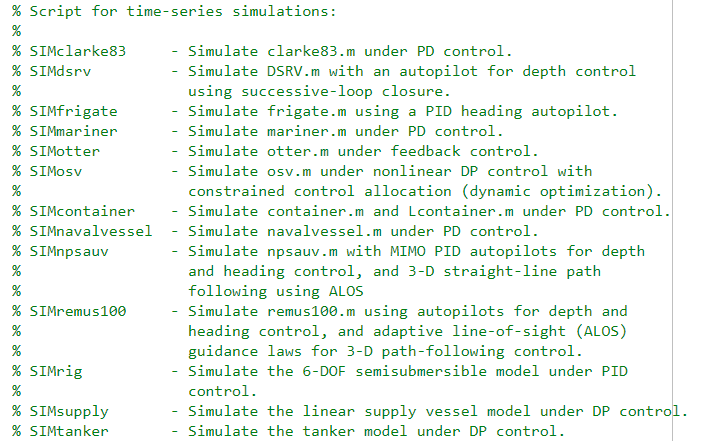
\includegraphics[width=0.5\linewidth]{img/contents_MSS.png}};
	\end{tikzpicture}
	
	
	\begin{tikzpicture}[remember picture,overlay]
		% \node[fill=blue!30, text=white, font=\large, rounded corners] 
		\node at (current page.north west) [xshift=9.5cm, yshift=-6.3cm] {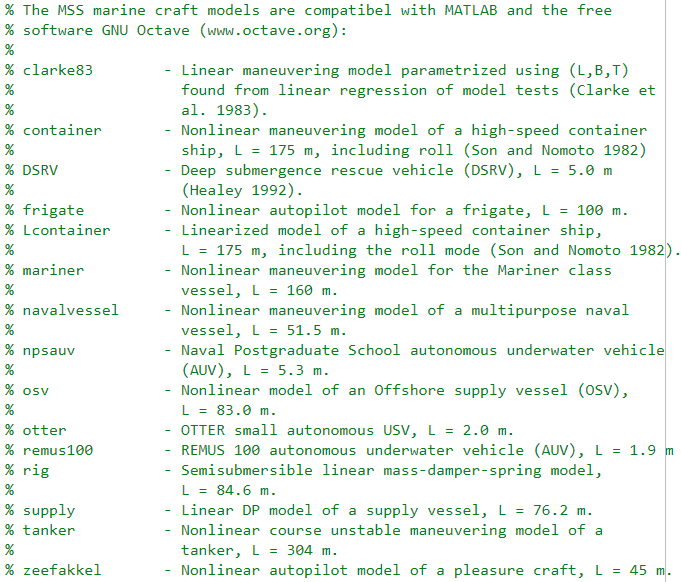
\includegraphics[width=0.5\linewidth]{img/contents_MSS1.png}};
	\end{tikzpicture}
\end{frame}

% =========================================
% =========================================


\begin{frame}{Numerical simulations}
	\framesubtitle{MSS Toolbox}
	Simulink models are constructed by MATLAB R2024
	
	\vspace{6cm}
	
	\begin{tikzpicture}[remember picture,overlay]
		% \node[fill=blue!30, text=white, font=\large, rounded corners] 
		\node at (current page.north west) [xshift=3cm, yshift=-5.5cm] {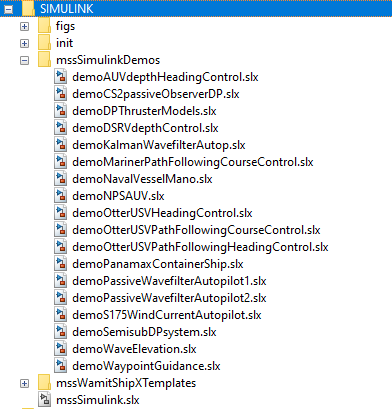
\includegraphics[width=0.5\linewidth]{img/contents_MSS2.png}};
	\end{tikzpicture}
	
	
	\begin{tikzpicture}[remember picture,overlay]
		% \node[fill=blue!30, text=white, font=\large, rounded corners] 
		\node at (current page.north west) [xshift=9.5cm, yshift=-4.3cm] {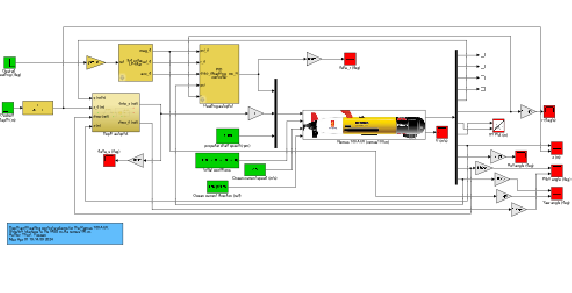
\includegraphics[width=0.5\linewidth]{img/contents_MSS3.png}};
	\end{tikzpicture}
	
	\begin{tikzpicture}[remember picture,overlay]
		% \node[fill=blue!30, text=white, font=\large, rounded corners] 
		\node at (current page.north west) [xshift=9.5cm, yshift=-7.3cm] {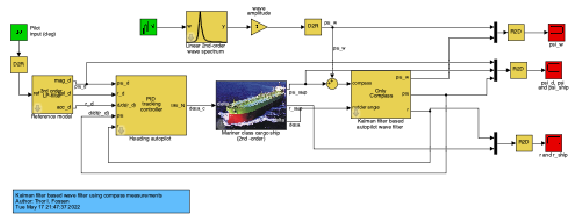
\includegraphics[width=0.5\linewidth]{img/contents_MSS4.png}};
	\end{tikzpicture}
\end{frame}




% =========================================
% =========================================


\begin{frame}{Numerical simulations}
	\framesubtitle{Example for ODIN}
	Forces distribution
	\vspace{3cm}
	%	\begin{tikzpicture}[remember picture,overlay]
		%		% \node[fill=blue!30, text=white, font=\large, rounded corners] 
		%		\node at (current page.north east) [xshift=-3cm, yshift=-5.5cm] 
		%		{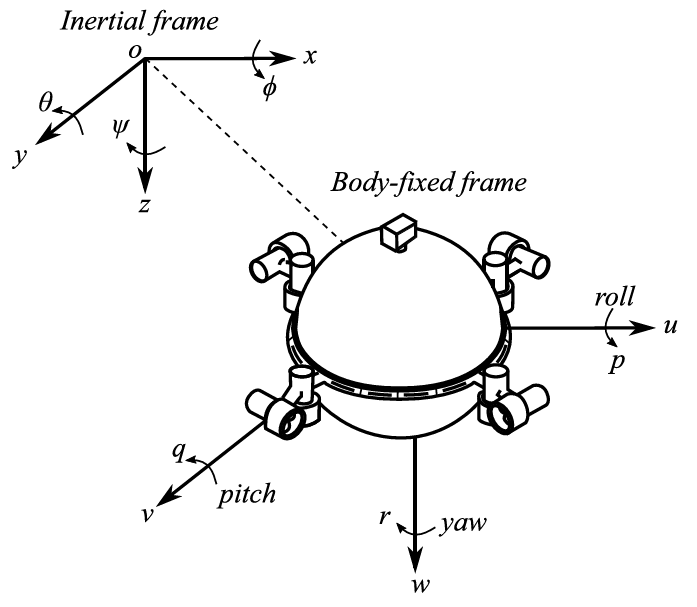
\includegraphics[width=0.4\linewidth]{img/ODIN.png}};
		%	\end{tikzpicture}
	
	\begin{tikzpicture}[remember picture,overlay]
		% \node[fill=blue!30, text=white, font=\large, rounded corners] 
		\node at (current page.north east) [xshift=-3cm, yshift=-5.5cm] 
		{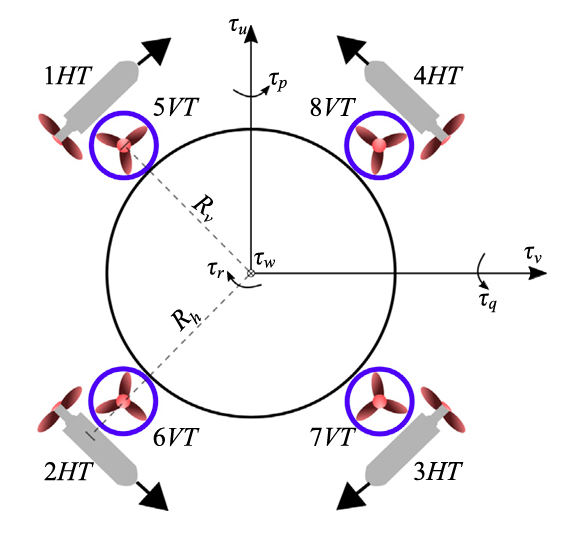
\includegraphics[width=0.4\linewidth]{img/ODIN1.png}};
	\end{tikzpicture}
	
	\begin{tikzpicture}[remember picture,overlay]
		% \node[fill=blue!30, text=white, font=\large, rounded corners] 
		\node at (current page.north east) [xshift=-9cm, yshift=-5.5cm] 
		{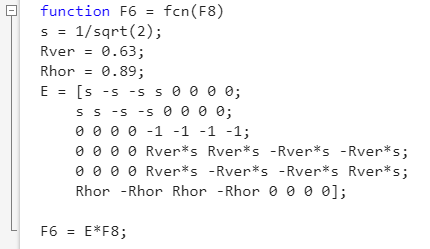
\includegraphics[width=0.5\linewidth]{img/force_distri.png}};
	\end{tikzpicture}
\end{frame}





% =========================================
% =========================================


\begin{frame}{Numerical simulations}
	\framesubtitle{Example for ODIN}
	%	\begin{tikzpicture}[remember picture,overlay]
		%		% \node[fill=blue!30, text=white, font=\large, rounded corners] 
		%		\node at (current page.north east) [xshift=-3cm, yshift=-5.5cm] 
		%		{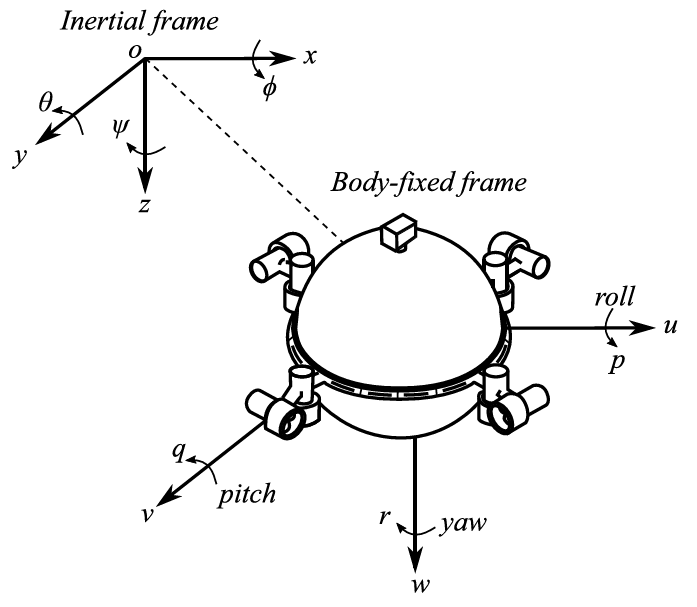
\includegraphics[width=0.4\linewidth]{img/ODIN.png}};
		%	\end{tikzpicture}
	Simulink simulation diagram
	\vspace{7cm}
	
	
	\begin{tikzpicture}[remember picture,overlay]
		% \node[fill=blue!30, text=white, font=\large, rounded corners] 
		\node at (current page.north east) [xshift=-6cm, yshift=-5.5cm] 
		{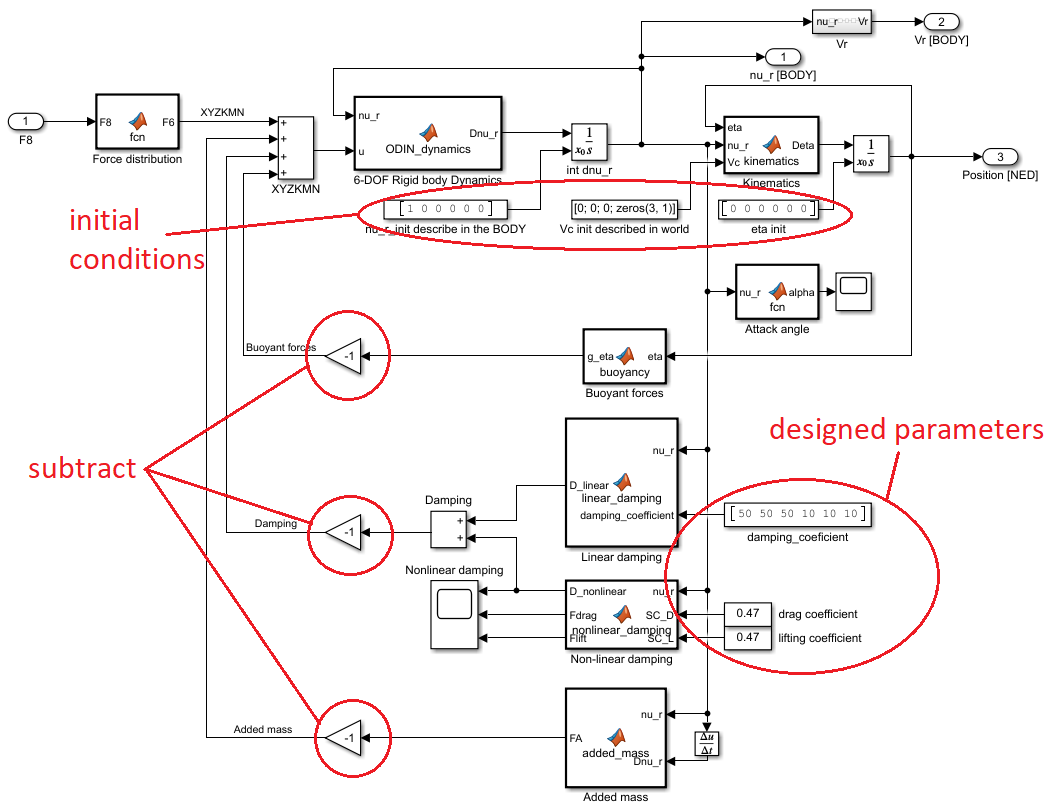
\includegraphics[width=0.8\linewidth]{img/ODIN_simulink.png}};
	\end{tikzpicture}
\end{frame}



% =========================================
% =========================================


\begin{frame}{Numerical simulations}
	\framesubtitle{Example for ODIN}
	Dynamics and kinematics m-file of ODIN
	\vspace{6cm}
	
	
	\begin{tikzpicture}[remember picture,overlay]
		% \node[fill=blue!30, text=white, font=\large, rounded corners] 
		\node at (current page.north east) [xshift=-9.5cm, yshift=-5.5cm] 
		{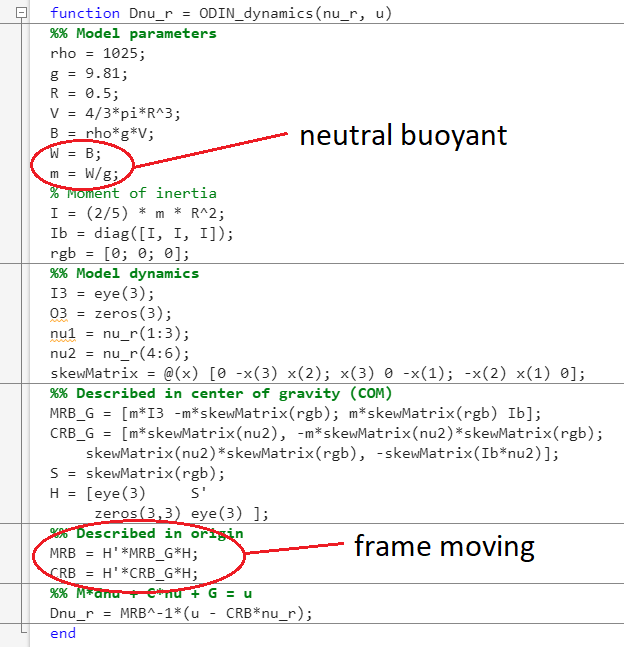
\includegraphics[width=0.5\linewidth]{img/ODIN_simulink1.png}};
	\end{tikzpicture}
	
	\begin{tikzpicture}[remember picture,overlay]
		% \node[fill=blue!30, text=white, font=\large, rounded corners] 
		\node at (current page.north east) [xshift=-3cm, yshift=-5.5cm] 
		{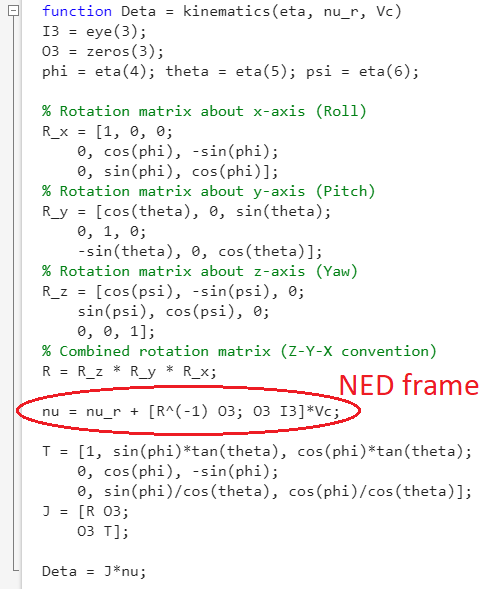
\includegraphics[width=0.4\linewidth]{img/ODIN_simulink2.png}};
	\end{tikzpicture}
	
\end{frame}




% =========================================
% =========================================


\begin{frame}{Numerical simulations}
	\framesubtitle{Example for ODIN}
	%	\begin{tikzpicture}[remember picture,overlay]
		%		% \node[fill=blue!30, text=white, font=\large, rounded corners] 
		%		\node at (current page.north east) [xshift=-3cm, yshift=-5.5cm] 
		%		{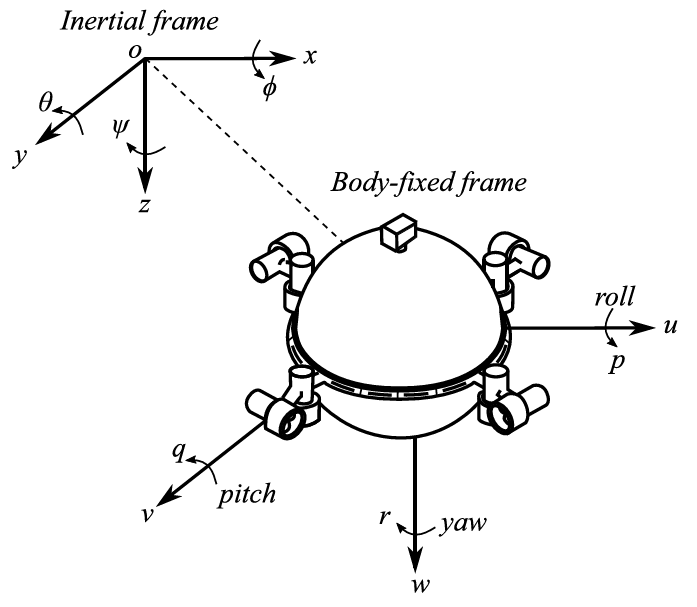
\includegraphics[width=0.4\linewidth]{img/ODIN.png}};
		%	\end{tikzpicture}
	Buoyancy forces
	\vspace{7cm}
	
	
	\begin{tikzpicture}[remember picture,overlay]
		% \node[fill=blue!30, text=white, font=\large, rounded corners] 
		\node at (current page.north east) [xshift=-6cm, yshift=-5.5cm] 
		{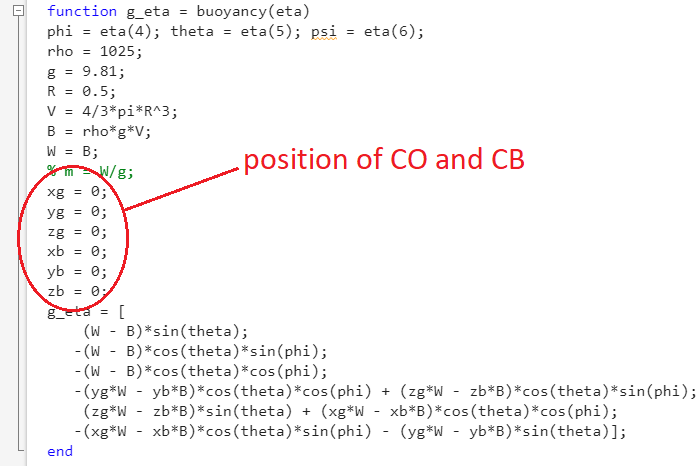
\includegraphics[width=0.8\linewidth]{img/ODIN_simulink3.png}};
	\end{tikzpicture}
\end{frame}



% =========================================
% =========================================


\begin{frame}{Numerical simulations}
	\framesubtitle{Example for ODIN}
	Damping terms
	\vspace{6cm}
	
	
	\begin{tikzpicture}[remember picture,overlay]
		% \node[fill=blue!30, text=white, font=\large, rounded corners] 
		\node at (current page.north east) [xshift=-8.5cm, yshift=-3.5cm] 
		{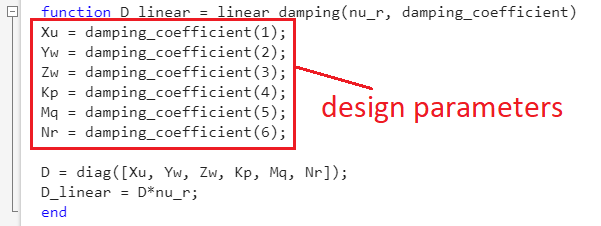
\includegraphics[width=0.6\linewidth]{img/ODIN_simulink4.png}};
	\end{tikzpicture}
	
	\begin{tikzpicture}[remember picture,overlay]
		% \node[fill=blue!30, text=white, font=\large, rounded corners] 
		\node at (current page.north east) [xshift=-4cm, yshift=-6.5cm] 
		{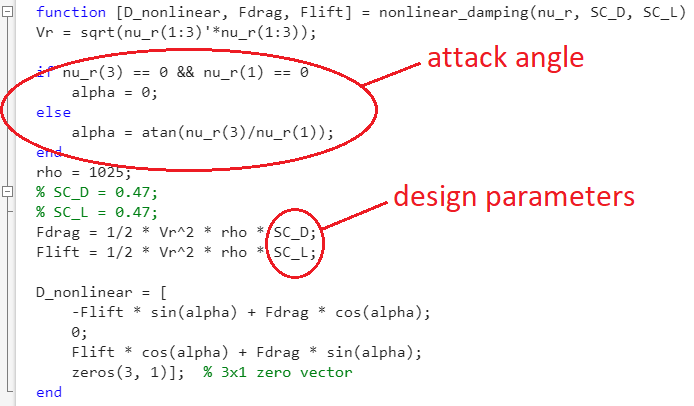
\includegraphics[width=0.6\linewidth]{img/ODIN_simulink5.png}};
	\end{tikzpicture}
	
\end{frame}





% =========================================
% =========================================


\begin{frame}{Numerical simulations}
	\framesubtitle{Example for ODIN}
	%	\begin{tikzpicture}[remember picture,overlay]
		%		% \node[fill=blue!30, text=white, font=\large, rounded corners] 
		%		\node at (current page.north east) [xshift=-3cm, yshift=-5.5cm] 
		%		{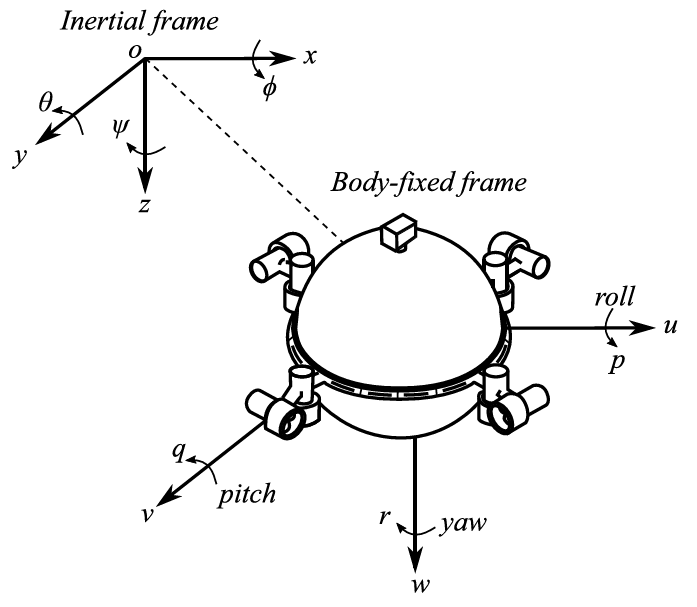
\includegraphics[width=0.4\linewidth]{img/ODIN.png}};
		%	\end{tikzpicture}
	Added mass
	\vspace{7cm}
	
	
	\begin{tikzpicture}[remember picture,overlay]
		% \node[fill=blue!30, text=white, font=\large, rounded corners] 
		\node at (current page.north east) [xshift=-6cm, yshift=-5.5cm] 
		{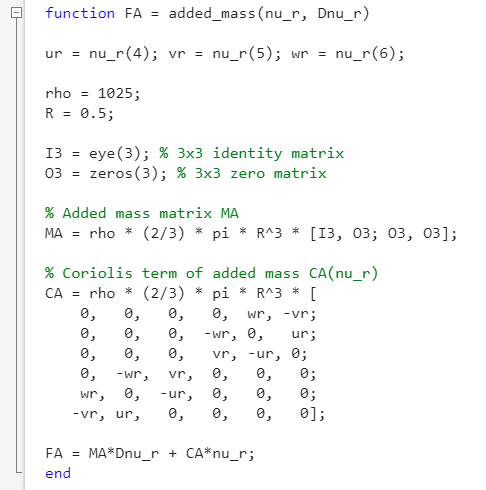
\includegraphics[width=0.6\linewidth]{img/ODIN_simulink6.png}};
	\end{tikzpicture}
\end{frame}



% =========================================
% =========================================



\begin{frame}{Numerical simulations}
	\framesubtitle{Example for ODIN}
	%	\begin{tikzpicture}[remember picture,overlay]
		%		% \node[fill=blue!30, text=white, font=\large, rounded corners] 
		%		\node at (current page.north east) [xshift=-3cm, yshift=-5.5cm] 
		%		{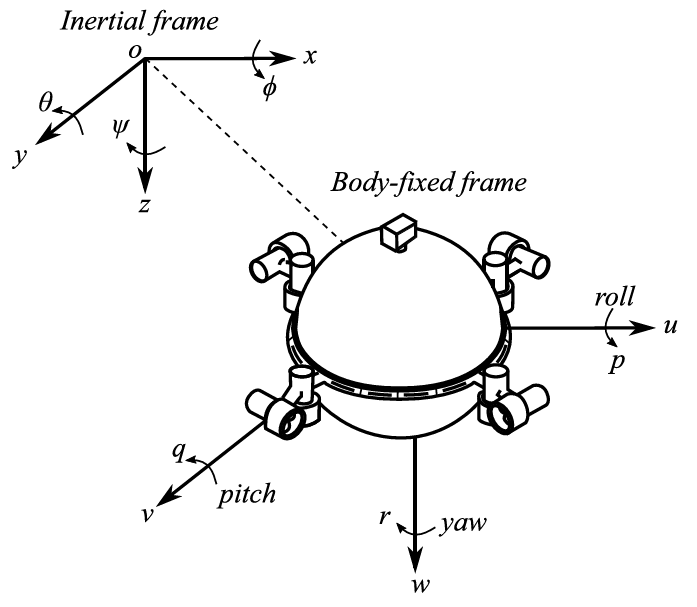
\includegraphics[width=0.4\linewidth]{img/ODIN.png}};
		%	\end{tikzpicture}
	Simple control structure
	\vspace{7cm}
	
	
	\begin{tikzpicture}[remember picture,overlay]
		% \node[fill=blue!30, text=white, font=\large, rounded corners] 
		\node at (current page.north east) [xshift=-6cm, yshift=-5.5cm] 
		{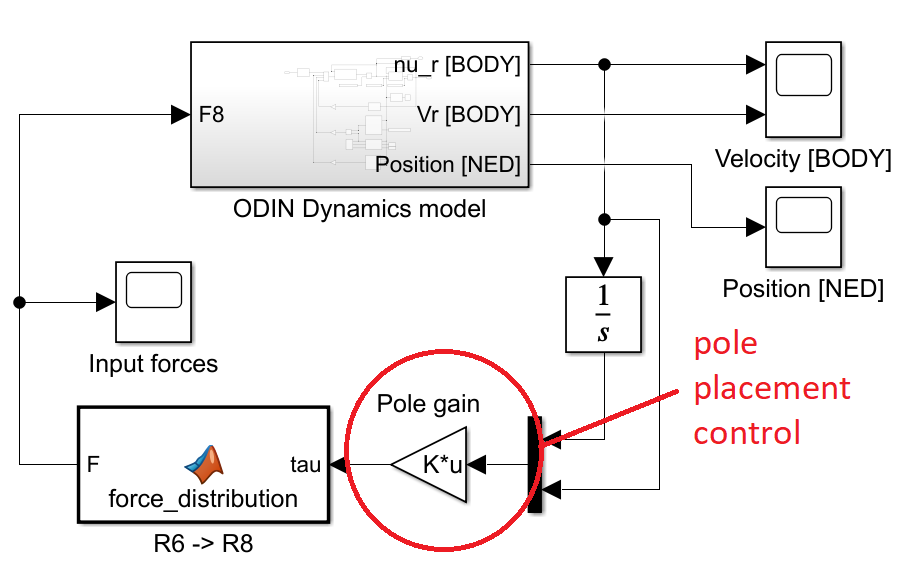
\includegraphics[width=0.8\linewidth]{img/ODIN_simulink7.png}};
	\end{tikzpicture}
\end{frame}

% =========================================
% =========================================



\begin{frame}{Numerical simulations}
	\framesubtitle{Example for ODIN}
	%	\begin{tikzpicture}[remember picture,overlay]
		%		% \node[fill=blue!30, text=white, font=\large, rounded corners] 
		%		\node at (current page.north east) [xshift=-3cm, yshift=-5.5cm] 
		%		{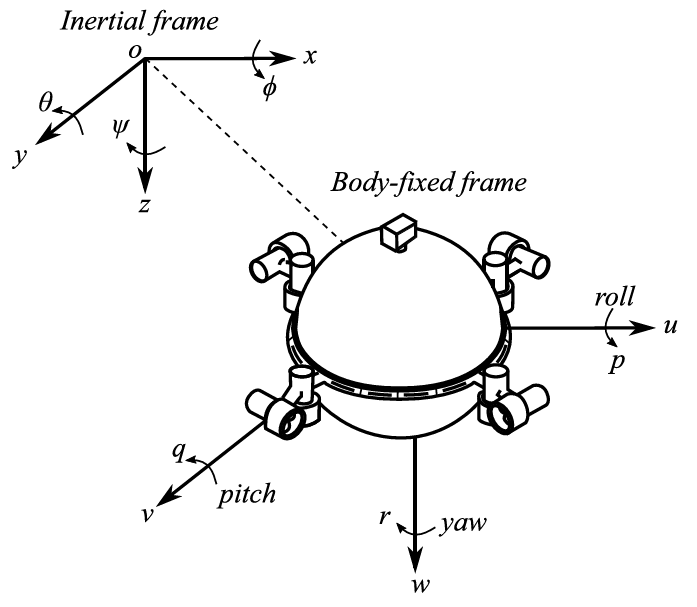
\includegraphics[width=0.4\linewidth]{img/ODIN.png}};
		%	\end{tikzpicture}
	Simple control structure
	\vspace{7cm}
	
	
	\begin{tikzpicture}[remember picture,overlay]
		% \node[fill=blue!30, text=white, font=\large, rounded corners] 
		\node at (current page.north east) [xshift=-6.5cm, yshift=-5.5cm] 
		{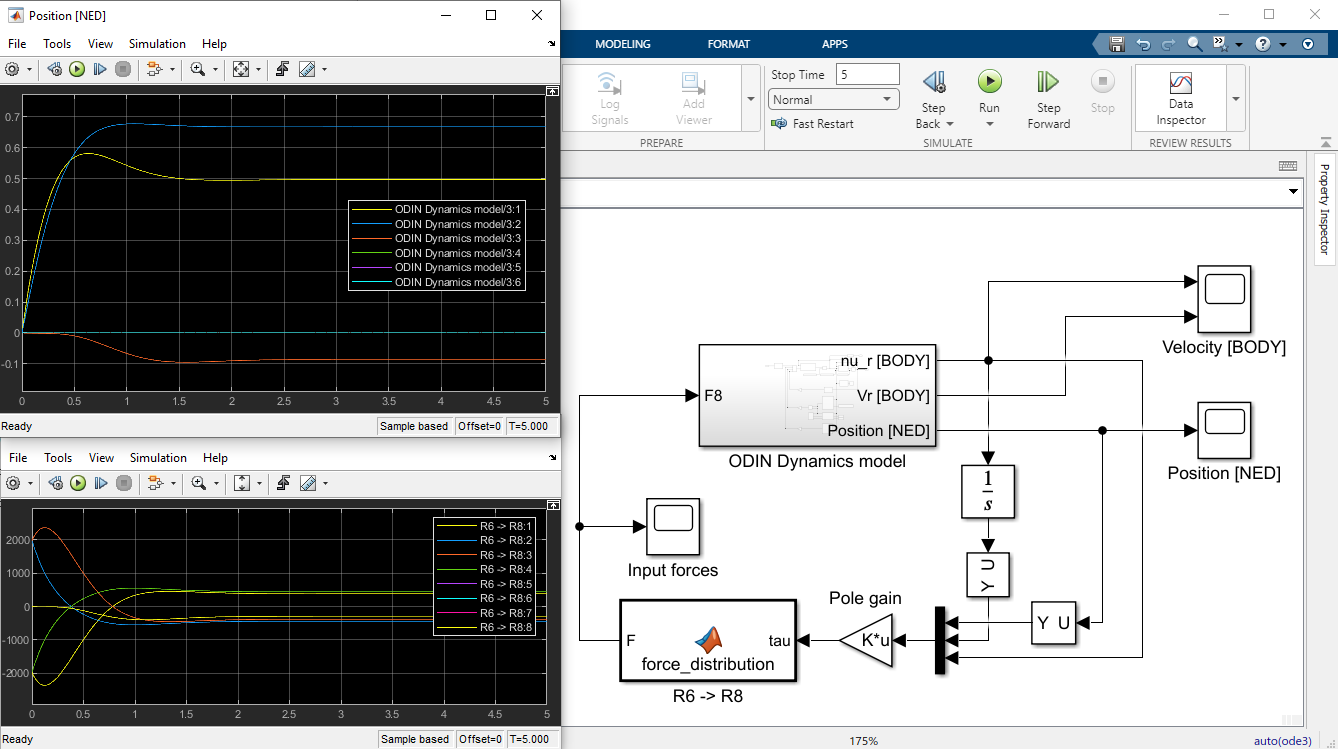
\includegraphics[width=\linewidth]{img/ODIN_simulink8.png}};
	\end{tikzpicture}
\end{frame}



% =========================================
% =========================================


\begin{frame}{Numerical simulations}
	\framesubtitle{Aerospace toolbox}
	Aerospace Toolbox provides standards-based tools and functions for analyzing the motion, mission, and environment of aerospace vehicles.
	
	\vspace{6cm}
	
	\begin{tikzpicture}[remember picture,overlay]
		% \node[fill=blue!30, text=white, font=\large, rounded corners] 
		\node at (current page.north west) [xshift=3cm, yshift=-6cm] {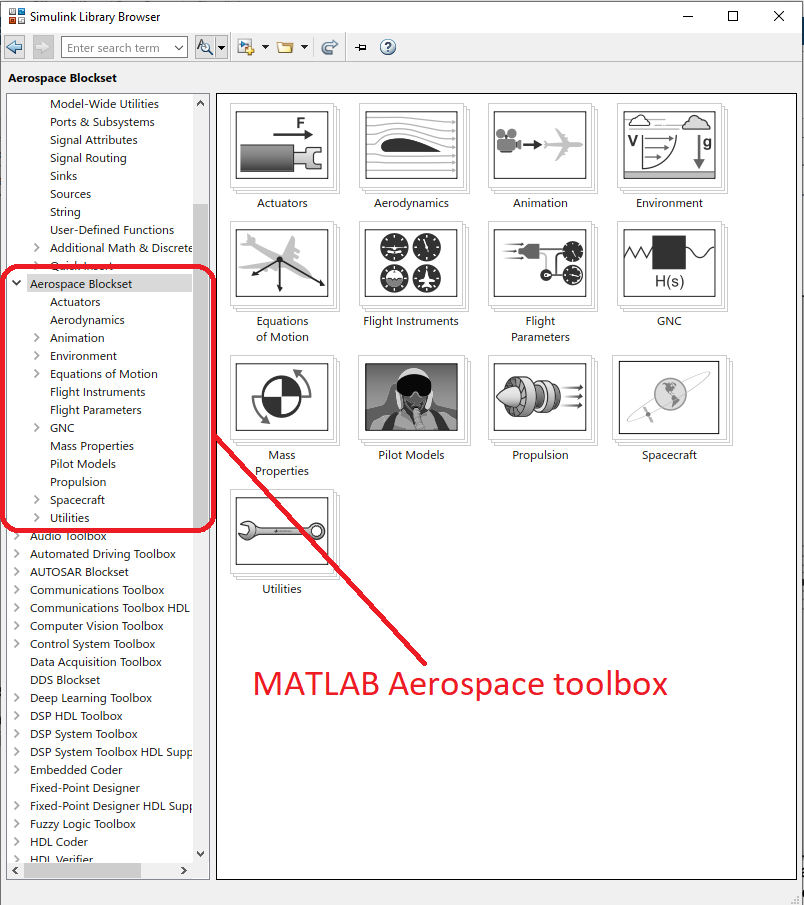
\includegraphics[width=0.5\linewidth]{img/aerospace toolbox.png}};
	\end{tikzpicture}
	
	
	\begin{tikzpicture}[remember picture,overlay]
		% \node[fill=blue!30, text=white, font=\large, rounded corners] 
		\node at (current page.north west) [xshift=9.5cm, yshift=-6cm] {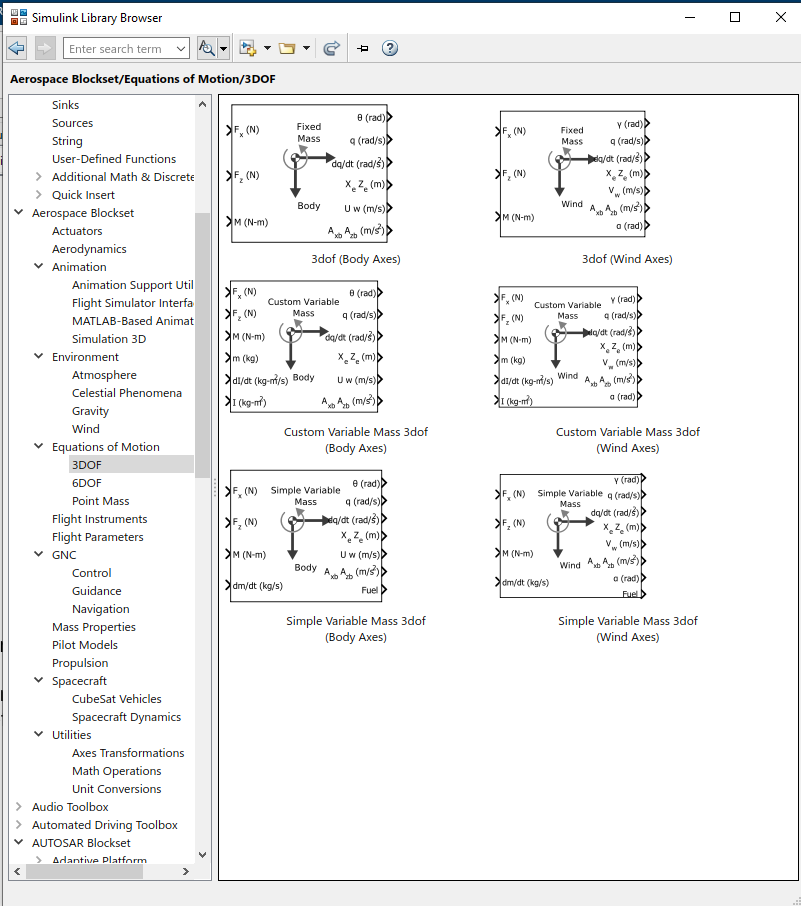
\includegraphics[width=0.5\linewidth]{img/aerospace toolbox 1.png}};
	\end{tikzpicture}
\end{frame}



% =========================================
% =========================================



\begin{frame}{Numerical simulations}
	\framesubtitle{Aerospace toolbox-aided simulation}
	A comparison of Aerospace toolbox and traditional numerical simulation
	
	\vspace{6.5cm}
	
	\begin{tikzpicture}[remember picture,overlay]
		% \node[fill=blue!30, text=white, font=\large, rounded corners] 
		\node at (current page.north east) [xshift=-6.5cm, yshift=-5.5cm] 
		{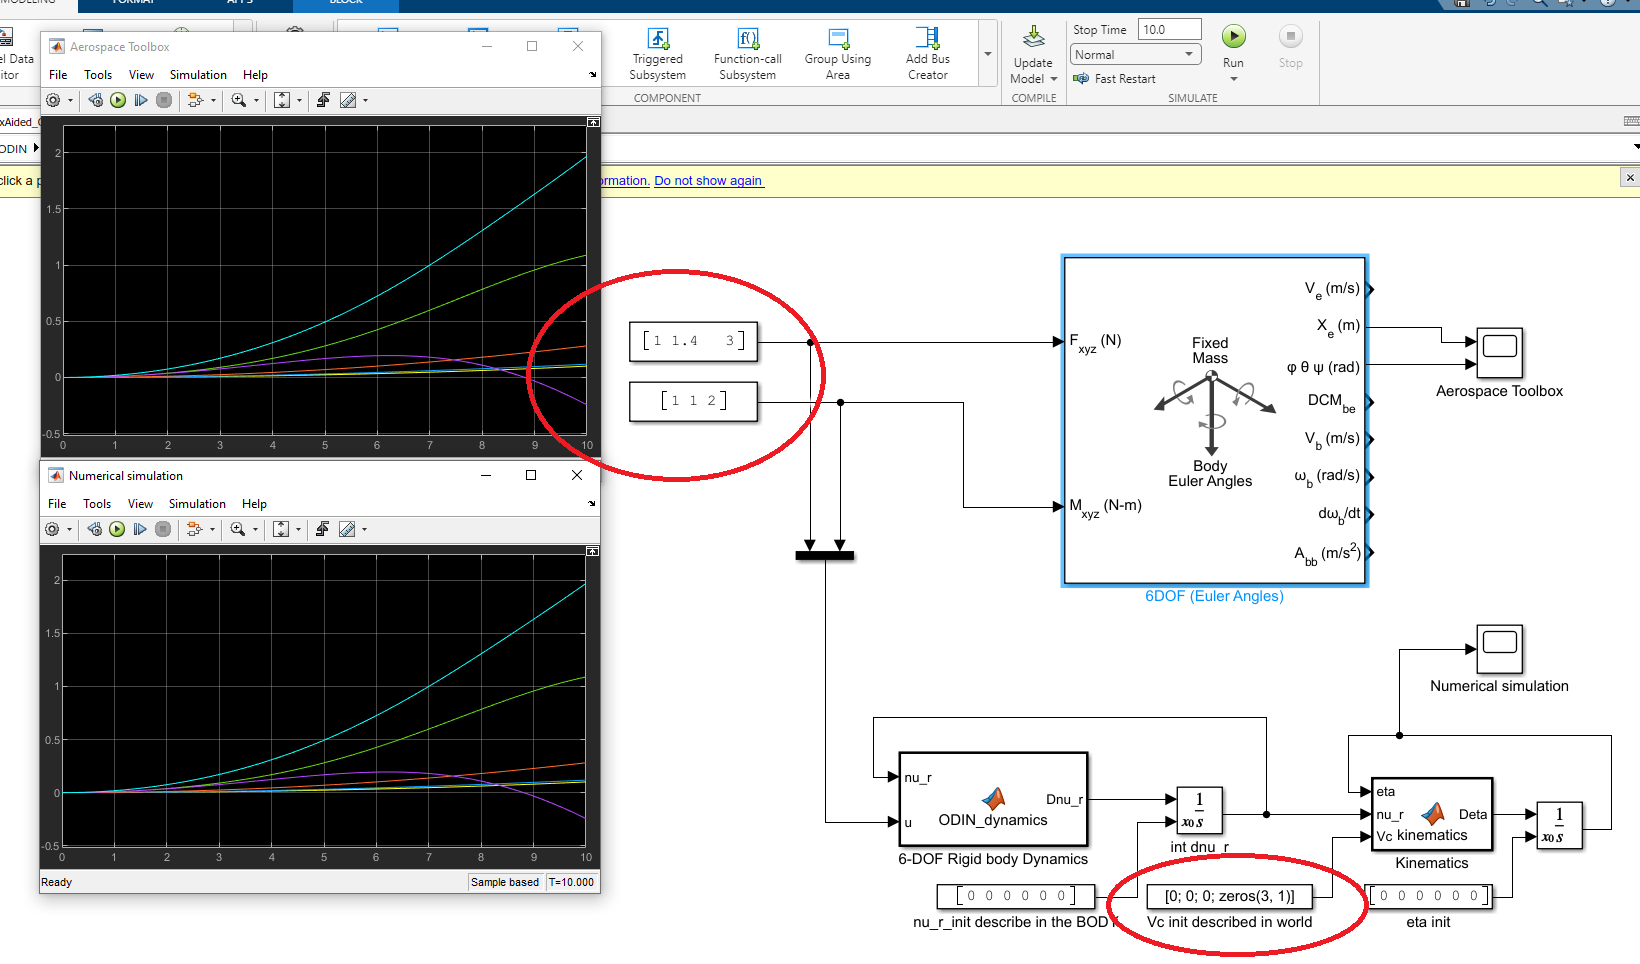
\includegraphics[width=0.9\linewidth]{img/aerospace toolbox 2.png}};
	\end{tikzpicture}
\end{frame}


% =========================================
% =========================================



\begin{frame}{Numerical simulations}
	\framesubtitle{Aerospace toolbox-aided simulation}
	Ocean current consideration.
	
	\vspace{6.5cm}
	
	\begin{tikzpicture}[remember picture,overlay]
		% \node[fill=blue!30, text=white, font=\large, rounded corners] 
		\node at (current page.north east) [xshift=-6.5cm, yshift=-5.5cm] 
		{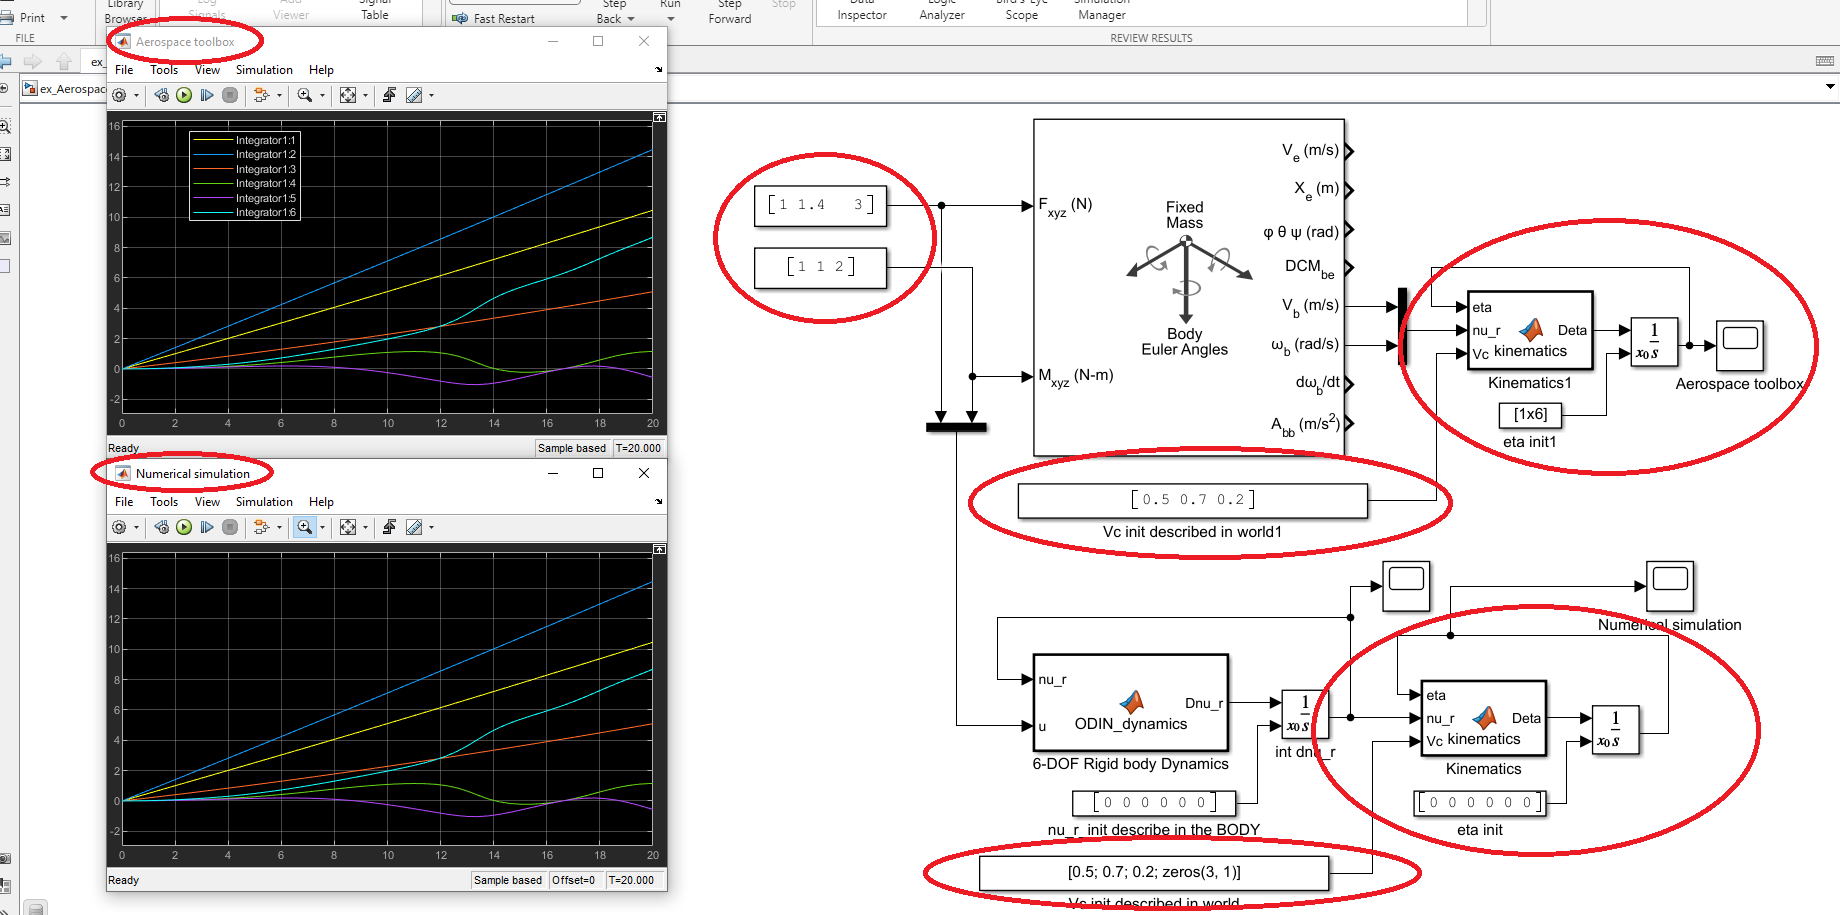
\includegraphics[width=\linewidth]{img/aerospace toolbox 3.png}};
	\end{tikzpicture}
\end{frame}


% =========================================
% =========================================





\begin{frame}{Numerical simulations}
	\framesubtitle{Aerospace toolbox-aided simulation}
	Modeling AUV with buoyant forces, nonlinear damping, and added mass.
	
	\vspace{6.5cm}
	
	\begin{tikzpicture}[remember picture,overlay]
		% \node[fill=blue!30, text=white, font=\large, rounded corners] 
		\node at (current page.north east) [xshift=-6.5cm, yshift=-5.5cm] 
		{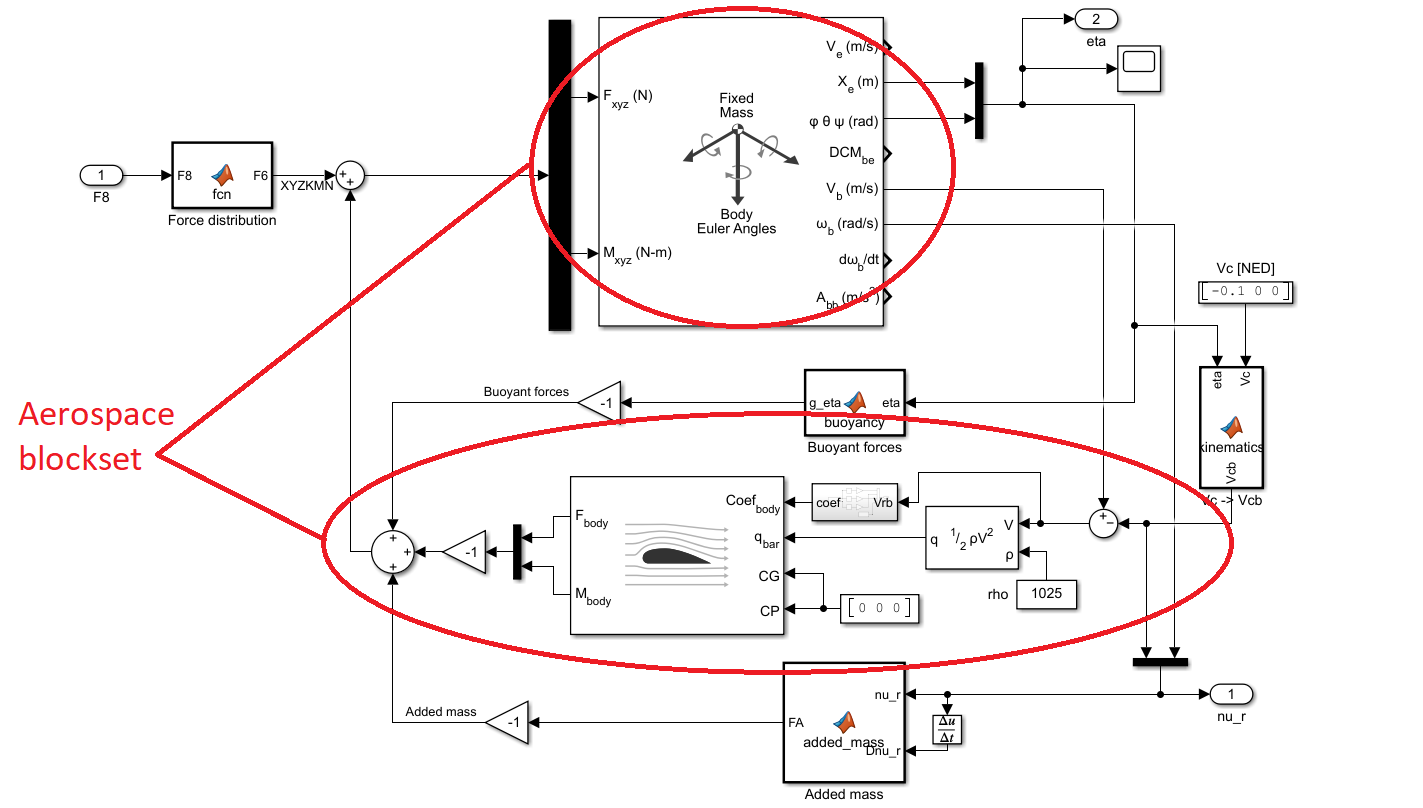
\includegraphics[width=\linewidth]{img/aerospace toolbox 4.png}};
	\end{tikzpicture}
\end{frame}



% =========================================
% =========================================




\begin{frame}{Numerical simulations}
	\framesubtitle{Aerospace toolbox-aided simulation}
	Simulation control structure
	
	\vspace{6.5cm}
	
	\begin{tikzpicture}[remember picture,overlay]
		% \node[fill=blue!30, text=white, font=\large, rounded corners] 
		\node at (current page.north east) [xshift=-6.5cm, yshift=-5.5cm] 
		{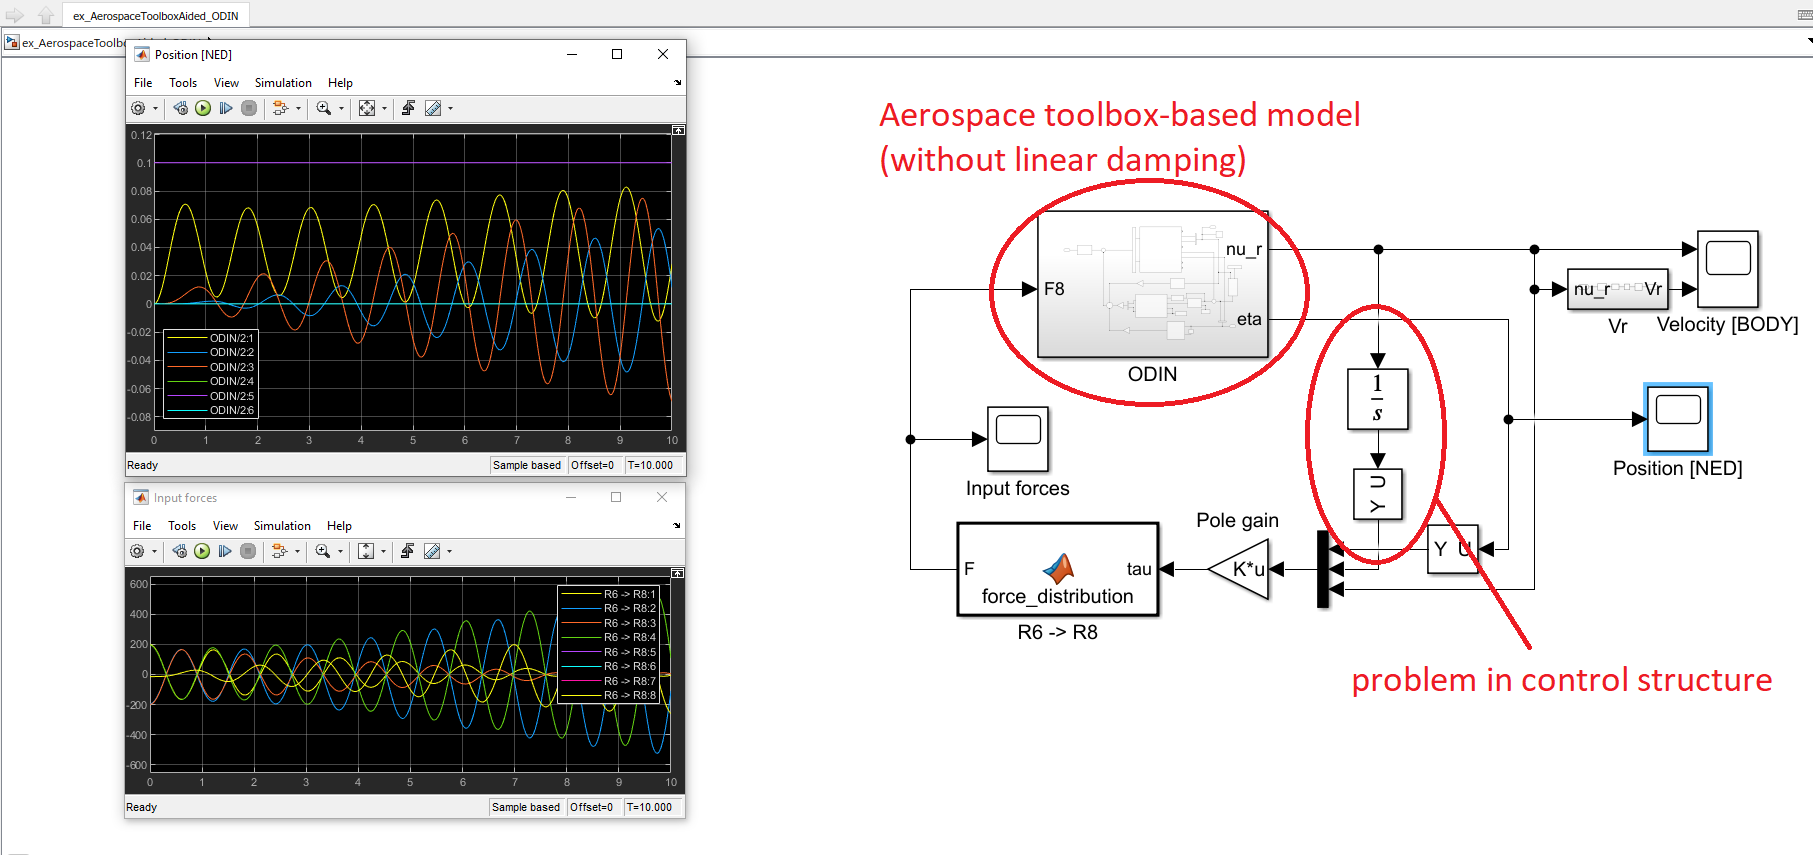
\includegraphics[width=\linewidth]{img/aerospace toolbox 5.png}};
	\end{tikzpicture}
\end{frame}


% =========================================
% =========================================



